\documentclass{report}

% Packages nécessaires
\usepackage[utf8]{inputenc}
\usepackage[T1]{fontenc}
\usepackage[english]{babel}
\usepackage{titlesec}
\usepackage{tocloft} % Gardé pour la personnalisation de la ToC
\usepackage{graphicx}
\usepackage{float} % pour l'option de placement [H]
\usepackage{minted} % pour la coloration syntaxique
\usepackage{wrapfig} % Pour l'enroulement du texte autour des images
\usepackage{array}


\usepackage{tabularx}
\usepackage{booktabs}
\usepackage{tikz}



% Mathématiques
\usepackage{amsmath, amssymb}
\usepackage{amsthm}
\usepackage{mdframed} % Package pour les cadres
\usepackage{algorithm}
\usepackage{algorithmic}

% Environnements pour les théorèmes, définitions et preuves
\newtheorem{theorem}{Théorème}[chapter]
\newtheorem{definition}{Définition}[chapter]
\newtheorem{example}{Exemple}[chapter]
\newtheorem{property}{Propriété}[chapter]

\newmdtheoremenv{boxedproperty}{Propriété}[section] % Crée un environnement encadré pour les propriétés

% Configuration de la page
\usepackage[a4paper, left=2.5cm, right=2.5cm, top=2.5cm, bottom=2.cm]{geometry}

% Pour avoir le petit dessin en bas à droite de chaque page
\usepackage{tikz} % Ajouté car nécessaire pour background avec tikzpicture
\usepackage{background}
\backgroundsetup{
scale=1,
angle=0,
opacity=1,
color=black,
contents={\begin{tikzpicture}[remember picture,overlay]
\node at ([xshift=-0.8in,yshift=0.8in] current page.south east) % Adjust the position of the logo.
{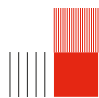
\includegraphics[scale=0.8]{images/pattern.png}}; % logo goes here
\end{tikzpicture}}
}

% Configuration des titres des sections et sous-sections
\titleformat{\chapter}[display]
  {\normalfont\huge\bfseries}{\chaptertitlename\ \thechapter}{20pt}{\Huge}
\titleformat{\section}
  {\normalfont\Large\bfseries}{\thesection}{1em}{}
\titleformat{\subsection}
  {\normalfont\large\bfseries}{\thesubsection}{1em}{}
\titleformat{\subsubsection}
  {\normalfont\normalsize\bfseries}{\thesubsubsection}{1em}{}

% --- MODIFICATIONS POUR SUBSUBSECTION ---
\setcounter{secnumdepth}{3} % Permet la numérotation des subsubsections
\setcounter{tocdepth}{3} % Permet l'affichage des subsubsections dans la table des matières
% --- FIN DES MODIFICATIONS POUR SUBSUBSECTION ---

% Configuration de la table des matières avec tocloft
\renewcommand{\cftchapfont}{\bfseries}
\renewcommand{\cftsecfont}{\normalfont}
\renewcommand{\cftsubsecfont}{\normalfont}
\renewcommand{\cftsubsubsecfont}{\normalfont} % Ajout pour la police du titre des subsubsections

\renewcommand{\cftchappagefont}{\bfseries}
\renewcommand{\cftsecpagefont}{\normalfont}
\renewcommand{\cftsubsecpagefont}{\normalfont}
\renewcommand{\cftsubsubsecpagefont}{\normalfont} % Ajout pour la police du numéro de page des subsubsections

\setlength{\cftbeforetoctitleskip}{0pt}
\setlength{\cftaftertoctitleskip}{10pt}
\renewcommand{\contentsname}{Table of Contents}

% Optionnel: ajuster l'indentation et la largeur du numéro pour subsubsection dans la ToC si besoin
\setlength{\cftsubsubsecindent}{6.5em} % Ajusté pour correspondre approximativement au PDF
\setlength{\cftsubsubsecnumwidth}{4.5em} % Ajusté pour correspondre approximativement au PDF

% Charger hyperref en dernier (ou presque)
\usepackage[colorlinks=true, linkcolor=blue, citecolor=green, urlcolor=blue]{hyperref}

\begin{document}

% Page de titre
\begin{titlepage}
    \centering

    % Minipages pour les logos
    \noindent % Assure qu'il n'y a pas d'indentation au début de la ligne
    \begin{minipage}{0.5\textwidth}
        
\includegraphics[width=0.5\linewidth]{images/logo_supcom.png} % Ajustez le chemin et la taille
    \end{minipage}%
    \hfill % Assure que les deux minipages seront poussés à l'extrême gauche et droite
    \begin{minipage}{0.5\textwidth}
        \flushright % Alignement à droite dans la minipage
        
\includegraphics[width=0.3\linewidth]{images/univ_carthage.png} % Ajustez le chemin et la taille
    \end{minipage}

    \vspace*{2cm} % Espace vertical de 2 cm
    {\Huge\bfseries Cloud of Things Scope Statement \par}
    \vspace{1cm}
    {\huge Smart Greenhouse\par}
    \vspace{2cm}
   \begin{center}
{\LARGE \textbf{Prepared by:} Marwen Bellili, Ghassen Zrigua, Maher Eloudi, Dhia Elhak Ezzeddini}\\[0.5cm]

{\LARGE \textbf{Supervised by:} Mr. Mohamed-Becha KAANICHE}
\end{center}

\begin{figure}[H]
    \centering
    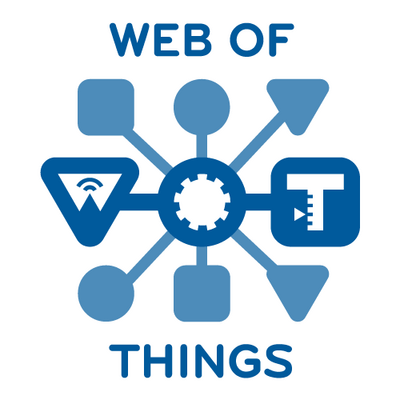
\includegraphics[width=0.6\textwidth]{images/webofthings.png}
\end{figure}

\vfill
{\Large \textbf{Higher School of Communications of Tunis} \par}
\vspace{1cm}
{\large \today \par}
\end{titlepage}

% Table des matières
\tableofcontents
\cleardoublepage % Pour que le chapitre suivant commence sur une page impaire

% Début du contenu du rapport
\chapter{Concept}
The concept of this project is to design and implement a \textbf{Smart Greenhouse System} based on Cloud of Things technologies, including the Internet of Things (IoT), cloud computing, and artificial intelligence (AI), to optimize plant growth conditions. The system will use sensors to continuously collect environmental data such as temperature, humidity, and water levels, as well as soil quality metrics (N, P, K). This information will be transmitted to the cloud for storage, processing, and analysis. The integration of an artificial intelligence component will allow for the automatic adjustment of actuators (fans, water pumps) to maintain an optimal environment, anticipate plant needs, and prevent unfavorable growth conditions.

\section{Problematic}
Traditional greenhouse management is often manual and imprecise, leading to inefficient water and energy consumption and vulnerability to environmental changes. It's difficult to maintain a consistent climate and soil quality, which can harm crop productivity. Furthermore, farmers often lack access to real-time data to make informed decisions. There is a pressing need for smart systems that can proactively monitor and control greenhouse environments, automating irrigation and ventilation processes while providing accurate information to farmers.

\section{Context of the Project}
This project is at the intersection of IoT, cloud computing, and AI. Recent advancements in sensors and mobile connectivity make it possible to capture agricultural data outside of lab environments. At the same time, cloud services provide the scalability and computational power necessary to process and analyze this data in real time. The integration of machine learning models opens the door to predicting growth conditions and triggering automated corrective actions. Within this technological context, our project demonstrates how the Cloud of Things can enable smarter, more sustainable agricultural solutions.

\section{Ambitions}
The ambitions of this project are to:
\begin{itemize}
    \item Improve crop yield and quality by maintaining optimal environmental conditions.
    \item Automate irrigation and ventilation tasks to reduce workload and human error.
    \item Optimize water and energy usage through data-driven controls.
    \item Provide farmers with real-time data insights via a dashboard.
    \item Explore the potential of machine learning in agriculture by predicting plant water and nutrient needs.
\end{itemize}

\chapter{Target Audience}
The Smart Greenhouse System is intended for two main groups:
\begin{itemize}
    \item \textbf{Commercial farmers and horticulturists}: Who require a reliable solution to optimize growing conditions and maximize their yield.
    \item \textbf{Gardening enthusiasts and individuals}: Who want to grow plants at home with an automated system, ensuring their health and well-being.
\end{itemize}

\chapter{Equipment}
The following equipment list is temporary and may evolve as the project progresses. It represents the initial hardware components considered for implementing the Smart Greenhouse System.

\begin{tabularx}{\linewidth}{|l|X|}
    \hline
    \textbf{Equipment} & \textbf{Description} \\
    \hline
    \textbf{Raspberry Pi 4/5} & Serves as the central processing and communication unit, handling sensor data aggregation and cloud connectivity. \\
    \hline
    \textbf{DHT11/DHT22 or SHT31 Sensors} & Measure the temperature and relative humidity of the greenhouse air. \\
    \hline
    \textbf{Water Level Sensor} & Detects the water level in a reservoir for irrigation (ultrasonic, capacitive, or analog float). \\
    \hline
    \textbf{NPK Soil Quality Sensor} & Measures the levels of Nitrogen (N), Phosphorus (P), and Potassium (K) in the soil. \\
    \hline
    \textbf{Relay} & Enables the control of actuators (fan, pumps) by switching the electrical supply. \\
    \hline
    \textbf{Electric Fan} & Used for ventilation and temperature control. \\
    \hline
    \textbf{Water Pump} & Actuates plant irrigation (pump for localized irrigation and a main pump). \\
    \hline
\end{tabularx}

\chapter{Functionalities}
\section{Sensor Data Acquisition}
The system will continuously collect environmental and soil data using the integrated sensors:
\begin{itemize}
    \item Temperature and humidity via the DHT or SHT sensor.
    \item Water level via the appropriate sensor.
    \item Nitrogen, Phosphorus, and Potassium (NPK) levels with the soil quality sensor.
\end{itemize}
Raw data will be processed locally on the Raspberry Pi for efficiency and securely transmitted to the cloud backend for storage and analysis.

\section{Mobile Application Development}
A mobile application, developed as a Progressive Web App (PWA) and Single Page Application (SPA), will serve as the main user dashboard. The app will provide the following functionalities:
\begin{itemize}
    \item Real-time visualization of sensor data (temperature, humidity, water level, NPK).
    \item Manual control of actuators (fan, pumps).
    \item Notifications and alerts if predefined thresholds are exceeded (e.g., temperature too high or low water level).
    \item A user-friendly interface accessible from various devices without requiring installation.
\end{itemize}

\section{Backend and Communication}
The backend will be developed using \textbf{Jakarta EE} as the middleware, providing a robust and scalable platform for processing and managing the data. Communication between the IoT devices and the backend will be handled by an \textbf{MQTT broker}, which is an efficient and lightweight messaging protocol ideal for IoT environments.

\section{Security}
The security of the system will be a top priority. \textbf{Identity and Access Management (IAM)} will be used to manage and secure access to the cloud resources and data. This includes authenticating devices and users, and authorizing their access to specific functionalities or data streams, ensuring patient privacy and compliance with health data regulations.

\chapter{Machine Learning Integration}
\section{Model Development}
The goal is to develop a compact and efficient machine learning model to analyze sensor data and make automated decisions. Depending on the chosen approach, the model will be used for:
\begin{itemize}
    \item \textbf{Irrigation Needs Prediction}: By using sensor data (soil moisture, temperature, etc.), the model can predict the plants' water needs and trigger the water pump.
    \item \textbf{Predictive Climate Control}: The model can anticipate temperature or humidity fluctuations and activate the fan or other control systems to maintain stable conditions.
\end{itemize}

\section{MLOps (Machine Learning Operations)}
An MLOps pipeline will be implemented to streamline the development, deployment, and monitoring of the predictive models. Its key features will include:
\begin{itemize}
    \item \textbf{Automated Training and Deployment}: The MLOps framework will train and update the model with new sensor data to ensure the accuracy of real-time predictions.
    \item \textbf{Performance Monitoring}: Continuous monitoring will track the model's effectiveness to detect drift and maintain its reliability.
    \item \textbf{Alerts and Notifications}: In case of critical conditions (e.g., risk of drought or overheating), the system will trigger immediate alerts for the user.
    \item \textbf{Data Management}: Secure data tracking and versioning will support model improvement.
    \item \textbf{Optimization and Feedback}: The model will be continuously refined based on real-world usage to optimize performance on local hardware.
\end{itemize}

\section{Dataset}
For model training, we will use the public dataset "IoT Agriculture 2024" available on Kaggle: \href{https://www.kaggle.com/datasets/wisam1985/iot-agriculture-2024/data?select=IoTProcessed_Data.csv}{Link}.

This dataset contains variables such as temperature, humidity, and soil quality data that are relevant to our project. We will explore two modeling approaches:
\begin{itemize}
    \item \textbf{Prophet}: A model developed by Facebook, suitable for time-series data, to predict water needs or temperature trends.
    \item \textbf{LSTM (Long Short-Term Memory)}: A type of recurrent neural network (RNN) capable of capturing long-term dependencies in time-series data, which could offer more accurate predictions.
\end{itemize}


\end{document}